%%%%%%%%%%%%%%%%%%%%%%%%%%%%%%%%%%%%%%%%%
% kaobookCJKsc
% LaTeX 文档类型
% Version 0.9.8 (2021/08/23)
%
% 原始模板来自:
% https://www.LaTeXTemplates.com
%
% 最新发布版本:
% https://github.com/fmarotta/kaobook
%
% 中文支持版本:
% https://github.com/xuehao/kaobookCJKsc
%
% 作者:
% Xue Hao (https://www.stickmind.com)
% Federico Marotta (federicomarotta@mail.com)
% Based on the doctoral thesis of Ken Arroyo Ohori (https://3d.bk.tudelft.nl/ken/en)
% and on the Tufte-LaTeX class.
% Modified for LaTeX Templates by Vel (vel@latextemplates.com)
%
% 许可:
% LPPL (see included MANIFEST.md file)
%
%%%%%%%%%%%%%%%%%%%%%%%%%%%%%%%%%%%%%%%%%

%----------------------------------------------------------------------------------------
%	kaobookCJKsc 文档类型示例与文档
%----------------------------------------------------------------------------------------

\documentclass[
    a4paper, % 页面设置
    fontsize=10pt, % 字号设置
    twoside=true, % 对偶数页和奇数页使用不同的布局(特别是,如果 twoside=true,边距列将始终在外面)
    open=any, % 如果 twoside=true,取消注释以强制新章节在任何页面上开始,而不仅仅是在正确(奇数)页面上
    chapterentrydots=true, % 在目录中,添加章节名到页码之间的圆点
    numbers=noenddot, % 注释章节号后的输出点; 此选项最常见的值是:enddot、noenddot 和 auto(请参阅 KOMAScript 文档以获得深入的解释)
]{styles/kaobookCJKsc}

%----------------------------------------------------------------------------------------
%	包以及文档配置,新项目可以直接复制粘贴
%----------------------------------------------------------------------------------------

% 加载排版包(不支持 chinese)
\usepackage{polyglossia}
\setmainlanguage{english}
\SetLanguageKeys{english}{indentfirst=true}
% 加载引号风格包(不支持 chinese)
\usepackage[style=english]{csquotes}
% 加载参考文献相关设置
\usepackage[style=gb7714-2015ms,backref=false]{styles/kaobiblioCJKsc} % 默认使用 GB 标准
\addbibresource{main.bib} % 参考文献文本
% 加载数学相关设置
\usepackage[framed]{styles/kaotheoremsCJKsc}
% 加载超链接相关设置
\usepackage{styles/kaorefsCJKsc}
% 加载平台中文字体及相关设置
\usepackage[testMathBox]{styles/kaoWinCJKsc}
% 加载测试包
\usepackage{blindtext}

% 图片路径
\graphicspath{{examples/documentation/images/}{images/}}
% 生成用于编译 索引 的文件
\makeindex[columns=3, title=索引, intoc]
% 生成用于编译 词汇表 的文件
\makeglossaries
\newglossaryentry{computer}{
	name=computer,
	description={一种可编程机器,它接收输入、存储和操作数据,并以有用的格式提供输出}
}

% Glossary entries (used in text with e.g. \acrfull{fpsLabel} or \acrshort{fpsLabel})
\newacronym[longplural={Frames per Second}]{fpsLabel}{FPS}{帧率}
\newacronym[longplural={Tables of Contents}]{tocLabel}{TOC}{目录}


% 生成用于编译 术语 的文件
\makenomenclature
% 每章开头重新给 边注 编号
\counterwithin*{sidenote}{chapter}
% 允许标题中出现 \\ 而不发出警告
\pdfstringdefDisableCommands{\let\\\empty}

%----------------------------------------------------------------------------------------
\begin{document}

%----------------------------------------------------------------------------------------
%	加载其他无法放在导言区的配置
%----------------------------------------------------------------------------------------
%%%%%%%%%%%%%%%无法放在导言区的设置%%%%%%%%%%%%%%%%%%%%
%目录中文名
\renewcommand{\contentsname}{目录}
\renewcommand{\listfigurename}{插图}
\renewcommand{\listtablename}{表格}
\renewcommand{\lstlistlistingname}{清单}
\renewcommand{\lstlistingname}{清单}
\renewcommand{\indexname}{索引}
\renewcommand{\bibname}{参考文献}
%其他中文名
\renewcommand{\pagename}{页}
\renewcommand{\chaptername}{章}
\renewcommand{\sectionname}{节}
\renewcommand{\subsectionname}{小节}
\renewcommand{\figurename}{图}
\renewcommand{\tablename}{表}
\renewcommand{\eqname}{公式}
\renewcommand{\defname}{定义}
\renewcommand{\assumname}{假设}
\renewcommand{\thmname}{定理}
\renewcommand{\propname}{命题}
\renewcommand{\lemmaname}{引理}
\renewcommand{\remarkname}{备注}
\renewcommand{\examplename}{例}
\renewcommand{\exercisename}{练习}
%引用语序
\renewcommand{\refpage}[1]{\hyperref[#1]{\textcolor{Blue}{第\xspace\pageref{page:#1}\xspace\pagename}}} % 第 84 页
\renewcommand{\refch}[1]{\hyperref[ch:#1]{\textcolor{Blue}{第\xspace\ref{ch:#1}\xspace\chaptername}}} % 第 7 章
\renewcommand{\nrefch}[1]{\hyperref[ch:#1]{\textcolor{Blue}{第\xspace\ref{ch:#1}\xspace\chaptername(\nameref{ch:#1})}}} % 第 7 章(数学)
\renewcommand{\refsec}[1]{\hyperref[sec:#1]{\textcolor{Blue}{第\xspace\ref{sec:#1}\xspace\sectionname}}}
\renewcommand{\nrefsec}[1]{\hyperref[sec:#1]{\textcolor{Blue}{第\xspace\ref{sec:#1}\xspace\sectionname(\nameref{sec:#1})}}}
\renewcommand{\refsubsec}[1]{\hyperref[subsec:#1]{\textcolor{Blue}{第\xspace\ref{subsec:#1}\xspace\subsectionname}}}
\renewcommand{\nrefsubsec}[1]{\hyperref[subsec:#1]{\textcolor{Blue}{第\xspace\ref{subsec:#1}\xspace\subsectionname(\nameref{subsec:#1})}}}
%脚注编号
% \renewcommand{\thefootnote}{\arabic{footnote}} % 1, 2, 3
% \renewcommand{\thefootnote}{\alph{footnote}} % a, b, c
% \renewcommand{\thefootnote}{\roman{footnote}} % i, ii, iii



%----------------------------------------------------------------------------------------
%	标题页
%----------------------------------------------------------------------------------------

\titlehead{嗨 kaobookCJKsc 在此}
\subject{一版在手,天下我有}

\title{基于 kaobookCJKsc 模板的\\示例与文档}
\subtitle{\nosat\textit{定制属于你的书籍}}

\author{薛浩}
\date{\zhtoday}

\publishers{绝绝子出版社}

%----------------------------------------------------------------------------------------

\frontmatter % 前置文档开始,使用罗马数字编号

%----------------------------------------------------------------------------------------
%	版权页
%----------------------------------------------------------------------------------------

\makeatletter
\uppertitleback{
	\textbf{内容提要}

	\bigskip
	介绍一种宽边排版的 \LaTeX 模板,常见于现代风格教科书。除了提供完整的开箱即用的特性,还允许用户自定义自己的特性。
}

\lowertitleback{
	\textbf{声明} \\
	您可以编辑此页面以满足您的需要。例如,有无版权声明以及其他一些信息。此页面基于 Ken Arroyo Ohori 论文的相应页面,改动很小。

	\medskip
	\textbf{版权没有,翻版不究} \\
	\cczero 本书使用 CC0 代码发布到公共领域。在法律允许的范围内,我放弃本作品的所有版权。

	要查看 CC0 代码的副本,请访问:\url{http://creativecommons.org/publicdomain/zero/1.0/}

	\medskip
	\textbf{出版说明} \\
	本文档基于 \href{https://sourceforge.net/projects/koma-script/}{\KOMAScript} 以及 \href{https://www.latex-project.org/}{\LaTeX} 并使用 \href{https://github.com/xuehao/kaobookCJKsc}{kaobookCJKsc} 模板。

	源码可以从这里下载:\url{https://github.com/xuehao/kaobookCJKsc}

	(欢迎贡献!)

	\medskip
	\textbf{版本} \\
	首次由\textbf{\@publishers}出版于\zhtoday
}
\makeatother

%----------------------------------------------------------------------------------------
%	致谢
%----------------------------------------------------------------------------------------

\dedication{
	世界的和谐体现在形式和数量上,心灵和灵魂以及自然哲学的所有诗意都体现在数学美的概念中。\\
	\flushright —— 达西·温特沃斯·汤普森
}

%----------------------------------------------------------------------------------------
%	标题页
%----------------------------------------------------------------------------------------

\maketitle % 注意,输出的标题页在此位置之前

%----------------------------------------------------------------------------------------
%	译者序
%----------------------------------------------------------------------------------------

\setchapterimage{seaside}
\chapter*{译者序} % 加星号防止多余书签
\addcontentsline{toc}{chapter}{译者序} % 添加到目录

无意间发现这份模板,感觉非常简约大方,所以就想尝试一下。不巧的是,作者没有考虑多语言问题,简体中文并没有默认支持。浅研究一下,就有了这个版本。目前基本满足日常所需,折服于 \LaTeX 的强大,是时候替换 Markdown 了。

下面简单说明一下 kaobookCJKsc 模板。首先,原则上\textbf{尽量减少对原模板的修改,以便于未来更新。}但是有些设置,一方面由于作者硬编码在样式文件中,另一方面由于很多包不支持中文,所以并不会自动翻译。为了处理这样的冲突,不得不拷贝一份,重新移植。主要工作有以下几个方面:

\begin{itemize}
    \item 为了区分原模板,所有文件增加了 CJKsc 后缀。
    \item 增加了类似 \texttt{kaoWinCJKsc.sty} 这样的配置包,尽可能将中文相关的配置以及平台依赖集中到这里。一来为跨平台提供便利,二来也能避免配置的杂乱无章。
    \item 为了项目结构的整洁,加入了 styles 子文件夹。
    \item 为了支持多平台,默认依赖 Google Noto 和 liberation 系列字体。
    \item 一些中文语序和英文相反,由于配置无法放在导言区或包内,单独增加一个 \texttt{config.tex} 文件保存,在正文中导入即可。
\end{itemize}

至此,一份漂亮的图书模板就做好了。本着够用就好的原则,没必要浪费太多时间在工具配置上。那么,万事具备,只欠东风,剩下的事情就交给你了。用好这份模板,多多创作吧!

\begin{flushright}
	\textit{薛浩}\hspace*{2.5em}

    \textit{\zhtoday}
\end{flushright}


%----------------------------------------------------------------------------------------
%	前言
%----------------------------------------------------------------------------------------

\setchapterstyle{plain} % 选择后续默认章节标题样式
\chapter*{前言}
\addcontentsline{toc}{chapter}{前言} % Add the preface to the table of contents as a chapter

I am of the opinion that every \LaTeX\xspace geek, at least once during
his life, feels the need to create his or her own class: this is what
happened to me and here is the result, which, however, should be seen as
a work still in progress. Actually, this class is not completely
original, but it is a blend of all the best ideas that I have found in a
number of guides, tutorials, blogs and tex.stackexchange.com posts. In
particular, the main ideas come from two sources:

\begin{itemize}
	\item \href{https://3d.bk.tudelft.nl/ken/en/}{Ken Arroyo Ohori}'s
	\href{https://3d.bk.tudelft.nl/ken/en/nl/ken/en/2016/04/17/a-1.5-column-layout-in-latex.html}{Doctoral
	Thesis}, which served, with the author's permission, as a backbone
	for the implementation of this class;
	\item The
		\href{https://github.com/Tufte-LaTeX/tufte-latex}{Tufte-Latex
			Class}, which was a model for the style.
\end{itemize}

The first chapter of this book is introductory and covers the most
essential features of the class. Next, there is a bunch of chapters
devoted to all the commands and environments that you may use in writing
a book; in particular, it will be explained how to add notes, figures
and tables, and references. The second part deals with the page layout
and design, as well as additional features like coloured boxes and
theorem environments.

I started writing this class as an experiment, and as such it should be
regarded. Since it has always been intended for my personal use, it may
not be perfect but I find it quite satisfactory for the use I want to
make of it. I share this work in the hope that someone might find here
the inspiration for writing his or her own class.

\begin{flushright}
	\textit{Federico Marotta}
\end{flushright}

\index{前言}

%----------------------------------------------------------------------------------------
%	目录 & 图片表格等列表
%----------------------------------------------------------------------------------------

\begingroup % 创建局部变量范围

\setlength{\textheight}{230\hscale} % 定义目录样式,手动修改页面高度

% Turn on compatibility mode for the etoc package
\etocstandarddisplaystyle % "toc display" as if etoc was not loaded
\etocstandardlines % "toc lines as if etoc was not loaded

\tableofcontents % 输出目录页
\listoffigures % 输出图片列表
\listoftables % 输出表格列表
\listoflstlistings % 输出清单(常为代码)列表
\endgroup % 结束局部变量范围

%----------------------------------------------------------------------------------------
%	术语
%----------------------------------------------------------------------------------------

\nomenclature{$c$}{真空惯性系中的光速}
\nomenclature{$h$}{普朗克常数}

\renewcommand{\nomname}{符号} % 重命名术语页面标题
\renewcommand{\nompreamble}{\noindent 以下列出正文中将会使用的几个符号:} % 术语表页面添加导言

\printnomenclature % 输出术语页面

%----------------------------------------------------------------------------------------

\mainmatter % 正文文档开始,重置页码并使用阿拉伯数字

%----------------------------------------------------------------------------------------
%	主体部分
%----------------------------------------------------------------------------------------

\setchapterstyle{kao} % 设置章节标题样式,为了统一,不要在章节内设置
\setchapterpreamble[u]{\margintoc}
\chapter{介绍}
\labch{介绍}

\section{灵感}

许多现代教科书都采用一种显眼的旁白排版,在旁白中可以展示图片,表格,标记等一切可以展示的东西。有证据表明,这种排版通过分离主体文本和辅助文本,有助于作者组织论述。同时,这些引用的辅助文本离主体文本非常近,方便读者查阅。

本文档并不是为了论证这种 1.5 栏宽边排版的好坏,因为已经有许多人在做类似的事情了。本文档的目的在于让读者用好 kaobookCJKsc 模板,同时也会介绍该类型的特点。

kaobookCJKsc 主要灵感来自于这篇\href{https://3d.bk.tudelft.nl/ken/en/2016/04/17/a-1.5-column-layout-in-latex.html}{博客},并且命名来自于原作者的名字 Ken Arroyo Ohori 首字母的缩写——原作者慷慨的授权我基于他的论文样式来创作这份模板。因此,如果你想用这种宽边排版制作你的书籍,可以去读一读他的博文。

你可能已经注意到了,另一个灵感来源是 \href{https://github.com/Tufte-LaTeX/tufte-latex}{Tufte-Latex} 模板。设计的本质其实是相似的,因为事实上,已有的这些模板已经足够好了,很难去彻底的提升。但是,我的想法是希望这份模板能比 Tufte-Latex 更灵活。比如,我尝试只用标准的包,并尽量减少从零设计。\sidenote{这也意味着理解并贡献这份模板会变得很容易。确实,许多特性还有待改进,如果感兴趣,就来 Github 主页吧。}因此,对于一些包提供的特性,如果你读了相关的文档,自定义应该非常容易。

在这本书里,我会介绍这份模板的主要特性,并提供如何使用和修改相关特性的信息。让我们开始吧。

\section{是什么}
\labsec{does}

\Class{kaobookCJKsc} 模板更多关注文档结构,而不是文档样式。正如著名的 \LaTeX 原则强调的,结构和样式应该尽可能分开。这份模板将只提供命令、环境以及一些用于定制的接口。实际上,有些样式相关的设置已经内置在模板中了,但用户仍可以自由定制。

\noindent 主要特性如下:

\begin{description}
	\item[页面排版] 降低了正文宽度以提高可读性,并且让出空间给文本注释以展示更多元素。
	\item[章节标题] 与 Tufte-Latex 不同的是,提供了多种章节标题,可以在本文档查看示例。
	\item[页面标题] 平铺整个页面,并且包含了留白。在双页模式下,将交替显示章节名和小节名。\sidenote{这也是区别于 Tufte-Latex 的地方。}
	\item[印刷材料] 已重新定义命令 \Command{frontmatter},\Command{mainmatter} 和 \Command{backmatter},以便在主要内容中自动具有宽边距,在前面和后面的内容中具有窄边距。但是,页面样式可以随时更改,即使是在文档的中间。
	\item[文本注释] 我们提供命令 \Command{sidenote} 和 \Command{marginnote} 将文本放在页边距中。\sidenote[][-2mm]{sidenote 有编号(像这样!),而 marginnotes 没有编号}
	\item[注释图表] \Environment{marginfigure} 和 \Environment{margintable} 是两个很有用的环境,允许你在页边距中放置数字和表格。(参见\reffig{marginmonalisa}).
	\item[注释目录] 既然我们有很宽的页边距,为什么不在其中添加一个小目录呢?参考 \Command{margintoc}。
	\item[超链接] 默认加载 \Package{hyperref},我们尝试以合理的方式添加书签;特别是,书签级别会在 \Command{appendix} 和 \Command{backmatter} 中自动重置。此外,我们还提供了一个小的包来简化文本其他部分的引用。
	\item[参考文献] 我们希望读者能够知道引用了什么,而不必每次都走到文档的末尾,因此引用会出现在页边空白处以及末尾,就像在 Tufte Latex 中一样。然而,与该模板不同的是,您可以根据自己的意愿自由定制引文。
\end{description}

\begin{marginfigure}[-3.5cm]
	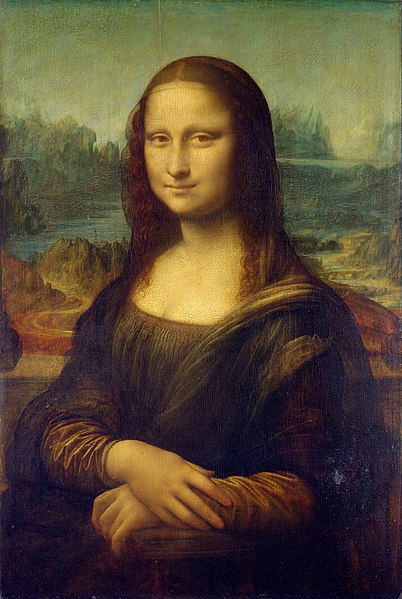
\includegraphics{monalisa}
	\caption[The Mona Lisa]{蒙娜丽莎\par\url{https://commons.wikimedia.org/wiki/File:Mona_Lisa,_by_Leonardo_da_Vinci,_from_C2RMF_retouched.jpg}}
	\labfig{marginmonalisa}
\end{marginfigure}

标题页、目录和前言的顺序可以很容易地更改,就像在任何 \LaTeX 文档中一样。此外,该模板基于 \KOMAScript 的 \Class{scrbook},因此它继承了原模板的所有优点。

\section{不是什么}
\labsec{doesnot}

正如预期的那样,该书的进一步定制将留给用户。可以肯定的是,每本书都有相似的旁注、页边数字等,但每本书都有自己独有的字体、目录风格、特殊环境等等。因此,除了类之外,我们只提供合理的默认值,但如果不需要这些特性,则可以忽略它们。这些特殊包位于样式目录中,其组织如下:

\begin{description}
	\item[kaoCJKsc.sty] 包含宏的最重要定义和页面排版规范。这是 \Class{kaobookCJKsc}	的核心。特殊功能包括:最常用的 \LaTeX 包已经自动加载;更改默认排版有一定的灵活性;一些特殊的环境(周围有彩色框、浮动或带计数的组件)是预定义的。\sidenote{参见\refch{引用}。}这是模仿 \Package{biblatex} 的。
	\item[kaorefsCJKsc.sty] 包含一些有用的命令来管理标签和引用,再次确保始终以一致的方式引用相同的元素。
	\item[kaotheoremsCJKsc.sty] 对于数学环境的样式,可以选择将其包装在彩色的 \Package{mdframed} 块中,如本文档所示,也可以不包装。
	\item[kaoWinCJKsc.sty] 提供 Windows 平台相关的设置。
	\item[config.tex] 存放一些无法放入样式文件的配置。
\end{description}

\marginnote[2mm]{大胆的用户可能会想编辑其中一些软件包。如果他们能给我寄来他们所能做到的例子,我将非常高兴!}

在本书的其余部分中,我将假设读者不是使用 \LaTeX 的新手,并参考本课程中使用的软件包的文档,了解其中已经解释的内容。此外,如果读者不喜欢默认设置,我假设读者愿意对提供的样式、环境和命令包进行少量编辑。

\section{如何用}
\labsec{howtouse}

先从 GitHub 仓库:\url{https://www.github.com/xuehao/kaobookCJKsc} 下载模板。

模板的使用方式有很多种。第一种是基于本文档项目,找到 main.tex 文件编辑即可;根据自己的需要删除部分文本,复制粘贴,重新创作。也可以基于另外两个 minimal 项目进行创作,他们是一个简化版本。无论如何,本文档项目都是最好的示例,你可以发现一些有用的特性,加入你自己的项目中。

对于想重头创建项目文档的用户,可以按照如下示例,先创建项目结构。默认使用时,文档结构如下所示\marginnote{译者注:注意 styles 文件夹不可以重命名,否则需要修改所有模板中的路径。}:

\begin{lstlisting}[style=kaolstplain]
	.
	├── styles
	│   ├── kaobiblioCJKsc.sty
	│   ├── kaobookCJKsc.cls
	│   ├── kaoCJKsc.sty
	│   ├── kaoWinCJKsc.sty
	│   ├── kaohandtCJKsc.cls
	│   ├── kaorefsCJKsc.sty
	│   ├── kaotheoremsCJKsc.sty
	│   └── config.tex
	├── main.tex                # 你的 LaTeX 文件
	├── Compiling.cmd
	└── Cleaning.cmd
\end{lstlisting}

编译同样需要使用命令行工具,切换到项目目录依次使用以下命令执行编译过程\marginnote[]{译者注:为了方便,译者提供了编辑好的编译脚本 \textbf{Compiling.cmd}。搭配 MiKTeX 发行版,已经在 Windows 10 平台上稳定使用。}:

\begin{lstlisting}[style=kaolstplain]
xelatex main                                  # 预编译模板
makeindex main.nlo -s nomencl.ist -o main.nls # 编译索引
makeindex main                                # 编译索引
biber main                                    # 编译参考文献
makeglossaries main                           # 编译字母表
xelatex main                                  # 再次编译模板
xelatex main                                  # 两到三次
xelatex main                                  # 防止边注错位
\end{lstlisting}

一般情况,按脚本顺序编译完即可,不会有错误。如有问题,可以去社区 \url{https://tex.stackexchange.org} 寻找答案,记得加上 kaobook 标签。当然,也可以在 GitHub 上创建 issues 或直接发邮件给我。

\section{\LaTeX 工作室}

众所周知,主流的 \LaTeX 发行版自带的编辑器非常难用。内置的编译流程也不太全面,无法做到一键编译。\marginnote{译者注:当然,搭配译者制作的一键编译工具,可以缓解一些不便之处!}为了实现高效编辑、简单编译、快速预览,这里推荐一套开源免费又轻巧好用的 \LaTeX 编译套装。推荐的方案是 \href{https://miktex.org/}{MiKTeX} 发行版,\href{https://code.visualstudio.com/}{Visual Studio Code} 编辑器搭配 \href{https://marketplace.visualstudio.com/items?itemName=James-Yu.latex-workshop}{\LaTeX\ Workshop} 插件。\marginnote{译者注:方案选择的首要原则是稳定,其次是跨平台,最后是免费。}

搭建自己的编译套装的前提是,\textbf{你必须了解你的编译工作流!}也就是说,针对你的文档项目,必须能使用前一小节介绍的命令行方式把完整的编译过程成功跑一遍。如果没有的话,大概率可以说明,你对 \LaTeX 编译工作流并不理解,后续对 Visual Studio Code 的配置也不可能正确。

在 Windows 平台下,要实现命令行完整编译的流程,需要安装以下几个工具:

\begin{lstlisting}[style=kaolstplain]
	\item 一款支持命令行工具的 \LaTeX 发行版,TeX Live 或 MiKTeX 等。
 	\item 默认支持的字体
 	\item 用于生成字母表的 Perl 工具
\end{lstlisting}

译者推荐安装 \href{https://miktex.org/}{MiKTeX} 发行版,选择 MiKTeX 有两个原因,其一是安装包很小,便于安装;其二是占用空间少,缺失的包会自动下载。Windows 平台安装完成后,打开命令提示符 CMD 输入以下命令测试(参见\reffig{marginmiktex}):

\begin{lstlisting}[style=kaolstplain]
	> xelatex --version
	MiKTeX-XeTeX 4.8 (MiKTeX 22.3)
	...
\end{lstlisting}

\begin{marginfigure}
	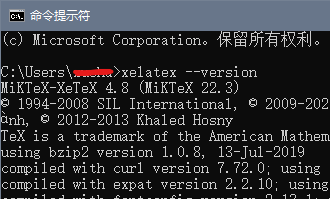
\includegraphics{miktex}
	\caption[MiKTeX]{MiKTeX}
	\labfig{marginmiktex}
\end{marginfigure}

简体中文模板默认使用美观、大方又开源的 \href{https://github.com/googlefonts/noto-cjk}{Google Noto} 字体。另外,原版英文字体需安装 liberation 系列字体,一并安装。\marginnote{译者注:字体备份 \url{https://pan.baidu.com/s/1r7qphMtlCdT9M3q26cokfA?pwd=uc75}}

除了字体,创建字母表页依赖 Perl 工具。为了后期的顺利编译,我们还需要安装 Perl,这里推荐安装 \href{https://strawberryperl.com/}{Strawberry Perl}。如果不需要字母表功能,可以不用安装,删除相关代码即可。

至此,已经可以愉快的使用命令行工具生成完整文档了。如上所述,我们继续安装 Visual Studio Code 以及其 \LaTeX Workshop 插件,以便实现高效编辑、自动编译、快捷预览等功能。

如果你之前使用命令行工具成功编译过你的项目,那么你一定会发现项目目录中多了很多杂七杂八的文件。每次删除都非常麻烦,一不小心还会删除自己的文件。\marginnote{译者注:对习惯命令行编译的用户,译者也慷慨地提供了一键清理工具 \textbf{Cleaning.cmd}。这也未尝不是一个好办法。}\LaTeX 项目需要多次编译,每次编译会依赖前一次生成的信息。对于我们这个工作流,编辑器插件虽然提供了自动清除功能,但由于其调用时机不确定,经常影响编译结果,所以不建议大家使用。因此,除非项目编译失败,编译过程中切记不要删除这些中间文件!只有确保文档创建成功后,再一次性清理。


\pagelayout{wide} % 无边距
\addpart{基础}
\pagelayout{margin} % 恢复边距

\setchapterpreamble[u]{\margintoc}
\chapter{文档类型选项}
\labch{文档类型选项}

本章将介绍最常用的选项,这些选项来自 \Class{scrbook} 以及 \Class{kaoCJKsc} 特有的部分。给模板设置选项将会改变其默认的行为,但要小心,有些选项会造成意想不到的结果……

\section{\Class{KOMA} 选项}

\Class{kaobookCJKsc} 模板基于 \Class{scrbook},因此,继承而来的设置选项同样可以生效。如果你有耐心,可以读一读 \KOMAScript 的使用手册。\sidenote{手册可以从这里下载 \url{https://ctan.org/pkg/koma-script?lang=en}。}实际上,建议读一下类似的使用手册,因为这些包含很多指导性的内容。

设置给模板的每一个 \KOMAScript 选项,会被自动加载。另外,在 \Class{kaobookCJKsc} 模板中,已经修改了部分默认的设置。比如,字体大小默认设置为 9.5pt,段落之间会使用空格分割\sidenote[][-7mm]{强调一下,段落间距默认设置为一半的行距:\Option{parskip} 值为 \enquote{half}。} ,并且会缩进 2 个汉字。

\section{\Class{kaoCJKsc} 选项}

未来计划加入一些设置段落格式的选项,以及边注位置的选项。\marginnote{译者注:原模板的段落是每行对齐的,\Class{kaobookCJKsc} 模板已经按中文习惯设置首行缩进。}借此机会,呼吁大家踊跃添加特性,重新设计现有特性,并能将结果发给我。可以在这里查看原版仓库 \url{https://github.com/fmarotta/kaobook}。

\begin{kaobox}[frametitle=\noindent 待办]
Implement the \Option{justified} and \Option{margin} options. To be consistent with the \KOMAScript style, they should accept a simple switch as a parameter, where the simple switch should be \Option{true} or \Option{false}, or one of the other standard values for simple switches supported by \KOMAScript. See the \KOMAScript documentation for further information.
\end{kaobox}

以上是使用 \Environment{kaobox} 的示例,将会在\nrefch{数学}详细介绍。本书会使用这样的块,标记将要实现的一些特性。

\section{其他值得关注的东西}

因实现的需要,一大堆包已经加载在该模板里了:

\begin{itemize}
	\item etoolbox
	\item calc
	\item xifthen
	\item xkeyval
	\item xparse
	\item xstring
\end{itemize}

对于大多数包,会在合适的时间去讨论。此刻,只提及一些用于段落格式调整的包(别忘了,未来这些可能被调整),主要包括以下这些:

\begin{itemize}
	\item ragged2e
	\item setspace
	\item hyphenat
	\item microtype
	\item needspace
	\item xspace
	\item xcolor (with options \Option{usenames,dvipsnames})
\end{itemize}

以上这些,有的不是针对段落格式的,但我们还是归到一起了。默认情况下,原模板主体文本和边注都是每行对齐的,而中文版主体文本调整为首行缩进,边注保持原样。

最后提醒一下,\Package{cleveref} 包与 \Class{kaobookCJKsc} 模板不兼容,请使用\nrefsec{hyprefs}讨论的命令替代。

\section{文档结构}

我们给 \Command{title} 和 \Command{author} 命令提供了可选参数,可以在前置文档中插入简短的文字。相应的,也提供了 \Command{@plaintitle} 和 \Command{@plainauthor} 命令,用于插入无样式的文字。pdf 属性由 \Option{pdftitle} 和 \Option{pdfauthor} 两个选项自动设置,也可以通过 hyperref 超链接设置具体值。\sidenote[][*-1]{由于这很重要,在此强调一下。如果 pdf 元数据被修改,编译时会设置为相应值;否则,元数据默认为文档的标题和作者。}

定义了两种页面排版 \Option{margin} 和 \Option{wide},以及两个页面样式 \Option{plain} 和 \Option{fancy}。排版只关注页边距,而样式指的是页眉和页脚。这些会在\nrefch{排版}讨论。\sidenote{目前只需要了解,\Option{margin} 排版有较宽的页边距,而 \Option{wide} 排版没有页边距。\Option{plain} 样式没有页眉页脚,而 \Option{fancy} 样式有页眉但是没有页脚。}

\Command{frontmatter},\Command{mainmatter} 和 \Command{backmatter} 三个命令重新定义以便自动切换页面的排版和样式。前置文档使用 \Option{wide} 排版和 \Option{plain} 样式。正文部分采用 \Option{margin} 排版和 \Option{fancy} 样式。附录部分保持不变;不过,我们可以使用 \Command{bookmarksetup\{startatroot\}} 命令,把章节书签等级设置为 root 级别,否则将会追加在前面的章节里。后置文档重新使用 \Option{wide} 排版,并重设了书签等级。

\setchapterpreamble[u]{\margintoc}
\chapter{文本标注}
\labch{文本标注}

边注是 1.5 栏宽边排版书籍的显著特性。确实,宽边距意味着更多的信息可以被显示出来,常用于放置带编号的边注、不带编号的边注、较小的章节目录、参考文献以及一些特别的块。

\section{带编号边注}

边注与脚注的区别就是其位置在页边距内,这样可读性会更高。插入一个边注可以使用命令 \Command{sidenote\{说明文本\}}。你可以使用命令 \Command{sidenote[记号]\{文本\}} 指定一个记号,\sidenote[O]{这条边注有一个 O !}也可以设置一个偏置距离,使文本向上或向下移动,完整语法如下:

\begin{lstlisting}[style=kaolstplain]
\sidenote[记号][偏置距离]{文本}
\end{lstlisting}

如果设置偏置距离,则记号的括号必须保留,内容可以为空。\sidenote{了解更多关于命令 \Command{sidenote} 的用法,请阅读 \Package{sidenotes} 包的文档。}

在 \Class{kaobookCJKsc} 模板中,我们从 \Package{snotez} 包中拷贝了一个特性:利用 \Command{baselineskip} 命令实现以行为单位的偏移。比如下面这样的语法会向上移动一行:

\begin{lstlisting}[style=kaolstplain]
\sidenote[][*-1]{边注文本}
\end{lstlisting}

刚才说过,边注由 \Package{sidenotes} 包提供,但此包又依赖 \Package{marginnote} 包。

\section{无编号边注}

这个命令,与前一节介绍的命令非常相似。可以用 \Command{marginnote[偏置]\{文本\}} 命令创建无编号的边注,同样包含偏置距离参数,以及基于 \Command{baselineskip} 命令实现的偏置行数参数,等等。\marginnote[-3cm]{虽然无编号边注命令来自 \Package{marginnote} 包,但是已经重新定义以便调整设置偏置参数的位置,目前该参数在边注文本之前设定,而原版命令在文本之后。同样,也基于 \Command{baselineskip} 增加了按行偏置的功能。这些设计目的是让所有命令有个统一的形式,防止太多命令需要记忆!}

\begin{lstlisting}[style=kaolstplain]
\marginnote[-12pt]{文本} or \marginnote[*-3]{文本}
\end{lstlisting}

\begin{kaobox}[frametitle=To Do]
A small thing that needs to be done is to renew the \Command{sidenote}
command so that it takes only one optional argument, the offset. The
special mark argument can go somewhere else. In other words, we want the
syntax of \Command{sidenote} to resemble that of \Command{marginnote}.
\end{kaobox}

我们加载了 \Package{marginnote}、\Package{marginfix} 和 \Package{placeins} 三个包。既然 \Package{sidenotes} 继承了 \Package{marginnote},我们之前讲的关于有编号边注同样适用于此。两种边注都做了轻微的调整(\texttt{\textbackslash renewcommand\{\textbackslash marginnote\linebreak vadjust\}\{3pt\}}),以对齐底部。重要的一点是,两种边注不指定偏置距离时,都采用垂直浮动布局。但是,一旦指定了偏置距离,浮动会禁用。少数情况下会出现一些问题,有时可以设置偏置距离为 0pt 以便消除浮动。

\section{脚注}

我们在这里讨论脚注,虽然它不显示在边注中,而且其作用也被边注替代。脚注强迫读者转移到页面的另一个区域。有证据表面,边注解决了这个问题。但无论如何,作为竞争者,我们保留了这个命令 \Command{footnote},以便你可以使用。\footnote{脚注以这样的形式存在,PDF 文件也会生成一个引用。}

\section{章节边注目录}
\labsec{martoc}

既然我们谈到了边注,这里再引入一个命令 \Command{margintoc} 用于在边注内生成一个小目录。和我们讨论过的其他命令一样,\Command{margintoc} 接受一个偏置距离参数,像这样:\Command{margintoc[offset]}。

命令可以用于文档任何位置,但我们认为在章节开头比较有意义。在这份文档里,我使用了 \KOMAScript 中的一个特性,并在导言区加入了这样的配置:

\marginnote{边注目录的字体和文档目录字体相同。}

\begin{lstlisting}[style=kaolstplain]
\setchapterpreamble[u]{\margintoc}
\chapter{Chapter title}
\end{lstlisting}

边注的空间是一个重要的资源,所以有可能需要在边注打印简短版的章节目录。于是节(小节)标题可能有三种:正文标题、文档目录标题、边注目录标题。这些不同版本可以使用如下命令同时设定:

\begin{lstlisting}[style=kaolstplain]
\section[alternative-title-for-toc]{title-as-written-in-text}[alternative-title-for-margintoc]
\end{lstlisting}

默认情况下,边注目录只包含节标题和小节标题,如果你只想展示节标题,添加如下命令到导言区:

\begin{lstlisting}[style=kaolstplain]
\setcounter{margintocdepth}{\sectiontocdepth}
\end{lstlisting}

\section{旁白列表}

On some occasions it may happen that you have a very short piece of code
that doesn't look good in the body of the text because it breaks the
flow of narration: for that occasions, you can use a
\Environment{marginlisting}. The support for this feature is still
limited, especially for the captions, but you can try the following
code:

\begin{marginlisting}[-1.35cm]
	\caption{An example of a margin listing.}
	\vspace{0.6cm}
	\begin{lstlisting}[language=Python,style=kaolstplain]
print("Hello World!")
	\end{lstlisting}
\end{marginlisting}

\begin{verbatim}
\begin{marginlisting}[-0.5cm]
	\caption{My caption}
	\vspace{0.2cm}
	\begin{lstlisting}[language=Python,style=kaolstplain]
	... code ...
	\end{lstlisting}
\end{marginlisting}
\end{verbatim}

Unfortunately, the space between the caption and the listing must be
adjusted manually; if you find a better way, please let me know.

Not only textual stuff can be displayed in the margin, but also figures.
Those will be the focus of the next chapter.

\setchapterpreamble[u]{\margintoc}
\chapter{图像与表格}

\footnotetext{The credits for the image above the chapter title go to:
	Bushra Feroz, CC~BY-SA~4.0, \url{https://commons.wikimedia.org/w/index.php?curid=68724647}}

\section{普通图像与表格}

Figures and tables can be inserted just like in any standard
\LaTeX\xspace document. The \Package{graphicx} package is already loaded
and configured in such a way that the figure width is equal to the
textwidth and the height is adjusted in order to maintain the original
aspect ratio. As you may have imagined, the captions will be
positioned\ldots well, in the margins. This is achieved with the help of
the \Package{floatrow} package.

Here is a picture of Mona Lisa (\reffig{normalmonalisa}), as an example.
The captions are formatted as the margin- and the side-notes; If you
want to change something about captions you can use the command
\Command{captsetup} from the \Package{caption} package. Remember that if
you want to reference a figure, the label must come \emph{after} the
caption!

\begin{figure}[hb]
	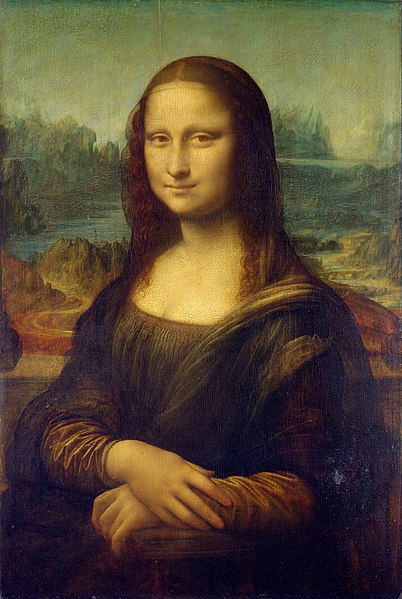
\includegraphics[width=0.45\textwidth]{monalisa}
	\caption[Mona Lisa, again]{It's Mona Lisa again. \blindtext}
	\labfig{normalmonalisa}
\end{figure}

While the format of the caption is managed by \Package{caption}, its
position is handled by the \Package{floatrow} package. Achieving this
result has been quite hard, but now I am pretty satisfied. In two-side
mode, the captions are printed in the correct margin.

Tables can be inserted just as easily as figures, as exemplified by the
following code:

\begin{lstlisting}[caption={Caption of a listing.}]
\begin{table}
\begin{tabular}{ c c c c }
	\toprule
	col1 & col2 & col3 & col 4 \\
	\midrule
	\multirow{3}{4em}{Multiple row} & cell2 & cell3 & cell4\\ &
	cell5 & cell6 & cell7 \\ &
	cell8 & cell9 & cell10 \\
	\multirow{3}{4em}{Multiple row} & cell2 & cell3 & cell4 \\ &
	cell5 & cell6 & cell7 \\ &
	cell8 & cell9 & cell10 \\
	\bottomrule
\end{tabular}
\end{table}
\end{lstlisting}

which results in the useless \reftab{useless}.

\begin{table}[ht]
\caption[A useless table]{A useless table.}
\labtab{useless}
\begin{tabular}{ c c c c }
	\toprule
	col1 & col2 & col3 & col 4 \\
	\midrule
	\multirow{3}{4em}{Multiple row} & cell2 & cell3 & cell4\\ &
	cell5 & cell6 & cell7 \\ &
	cell8 & cell9 & cell10 \\
	\multirow{3}{4em}{Multiple row} & cell2 & cell3 & cell4 \\ &
	cell5 & cell6 & cell7 \\ &
	cell8 & cell9 & cell10 \\
	\bottomrule
\end{tabular}
\end{table}

I don't have much else to say, so I will just insert some blind text.
\blindtext

\section{旁白图像与表格}

Marginfigures can be inserted with the environment
\Environment{marginfigure}. In this case, the whole picture is confined
to the margin and the caption is below it. \reffig{marginmonalisa} is
obtained with something like this:

\begin{lstlisting}[caption={Another caption.}]
\begin{marginfigure}
	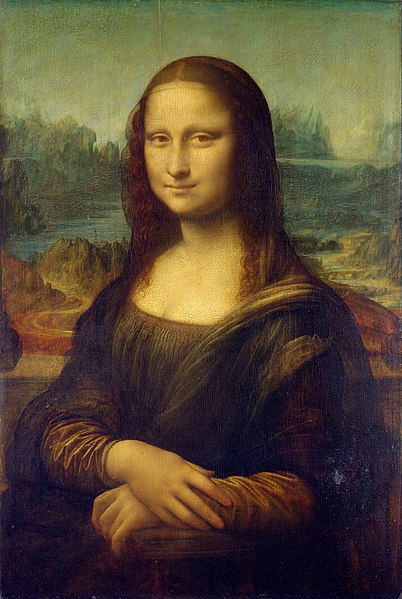
\includegraphics{monalisa}
	\caption[The Mona Lisa]{The Mona Lisa.}
	\labfig{marginmonalisa}
\end{marginfigure}
\end{lstlisting}

There is also the \Environment{margintable} environment, of which
\reftab{anotheruseless} is an example. Notice how you can place the
caption above the table by just placing the \Command{caption} command
before beginning the \Environment{tabular} environment. Usually, figure
captions are below, while table captions are above. This rule is also
respected for normal figures and tables: the captions are always on the
side, but for figure they are aligned to the bottom, while for tables to
the top.

\begin{margintable}
\caption[Another useless table]{Another useless table.}
\labtab{anotheruseless}
\raggedright
\begin{tabular}{ c c c c }
	\hline
	col1 & col2 & col3 \\
	\hline
	\multirow{3}{4em}{Multiple row} & cell2 & cell3 \\ & cell5 & cell6
	\\ & cell8 & cell9 \\ \hline
\end{tabular}
\end{margintable}

Marginfigures and tables can be positioned with an optional offset
command, like so:

\begin{lstlisting}
\begin{marginfigure}[offset]
	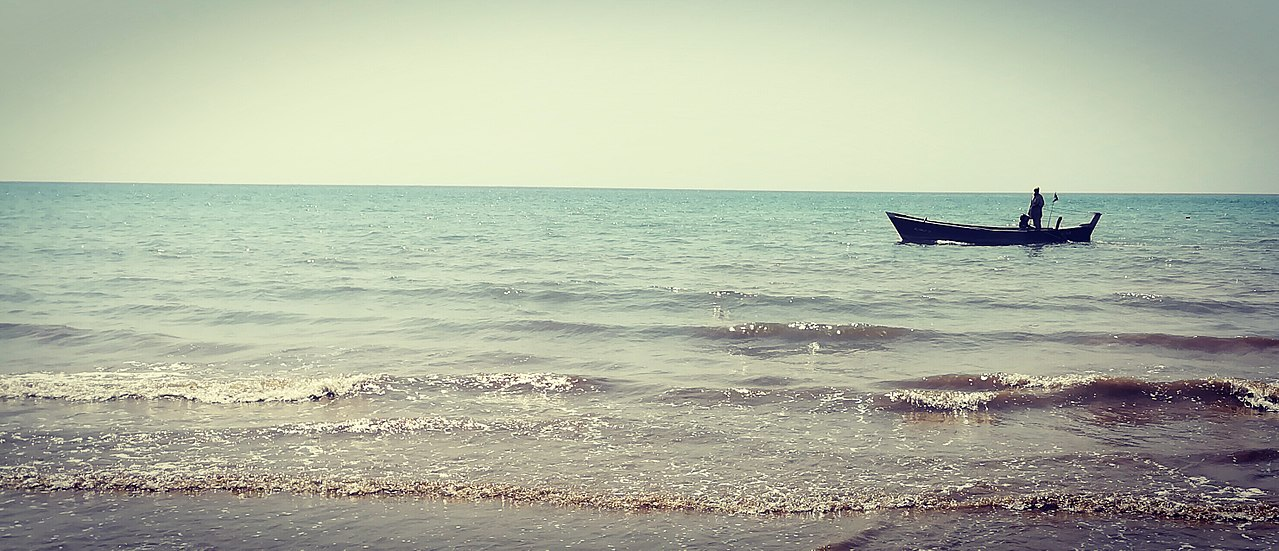
\includegraphics{seaside}
\end{marginfigure}
\end{lstlisting}

Offset ca be either a measure or a multiple of \Command{baselineskip},
much like with \Command{sidenote}, \Command{marginnote} and
\Command{margintoc}.\todo{Improve this part.} If you are wondering how I
inserted this orange bubble, have a look at the \Package{todo} package.

\section{超宽图像与表格}

With the environments \Environment{figure*} and \Environment{table*} you
can insert figures which span the whole page width. For example, here
are a wide figure and a wide table.

\begin{figure*}[h!]
	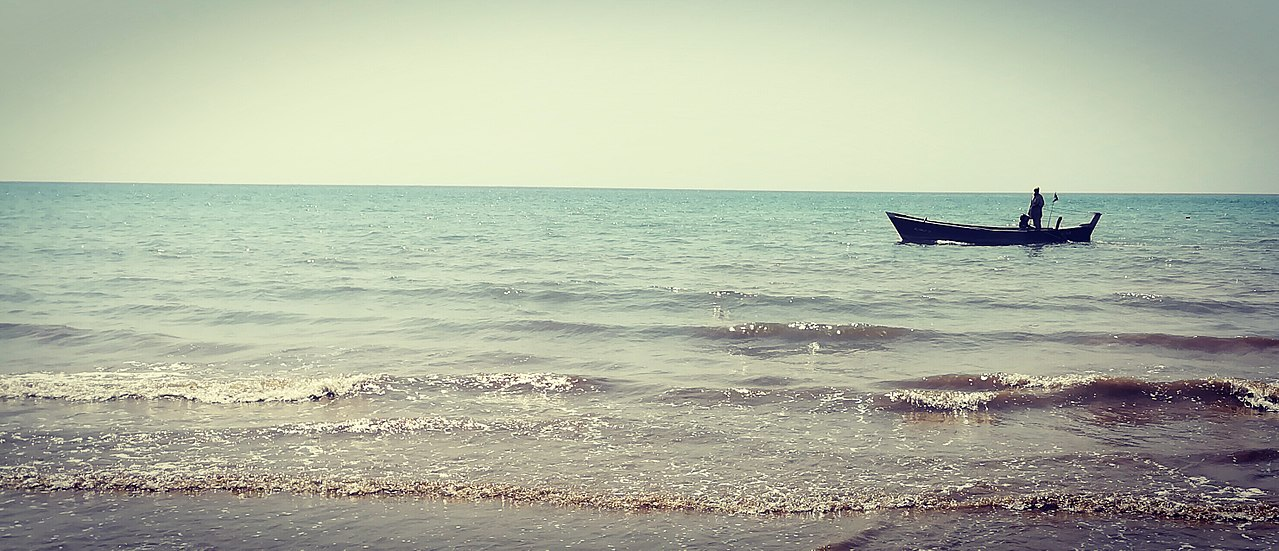
\includegraphics{seaside}
	\caption[A wide seaside]{A wide seaside, and a wide caption.
		Credits: By Bushra Feroz, CC BY-SA 4.0, \url{https://commons.wikimedia.org/w/index.php?curid=68724647}}
\end{figure*}

\begin{table*}[h!]
    \caption{A wide table with invented data about three people living in the UK. Note that wide figures and tables are centered and their caption also extends into the margin.}
    \begin{tabular}{p{2.0cm} p{2.0cm} p{2.0cm} p{2.0cm} p{2.0cm} p{2.0cm} p{1.5cm}}
        \toprule
        Name    & Surname   & Job       & Salary           & Age   & Height    & Country \\
        \midrule
        Alice   & Red       & Writer    & 4.000 \pounds    & 34    & 167 cm     & England \\
        Bob     & White     & Bartender & 2.000 \pounds    & 24    & 180 cm     & Scotland \\
        Drake   & Green     & Scientist & 4.000 \pounds    & 26    & 175 cm     & Wales \\
        \bottomrule
    \end{tabular}
\end{table*}

It is the user's responsibility to adjust the width of the table, if
necessary, until it is aesthetically pleasing. The previous table was
obtained with the following code:

\begin{lstlisting}[caption=How to typeset a wide table]
\begin{table*}[h!]
    \caption{A wide table with invented data about three people living in the UK. Note that wide figures and tables are centered and their caption also extends into the margin.}
    \begin{tabular}{p{2.0cm} p{2.0cm} p{2.0cm} p{2.0cm} p{2.0cm} p{2.0cm} p{1.5cm}}
        \toprule
        Name    & Surname   & Job       & Salary           & Age   & Height    & Country \\
        \midrule
        Alice   & Red       & Writer    & 4.000 \pounds    & 34    & 167 cm     & England \\
        Bob     & White     & Bartender & 2.000 \pounds    & 24    & 180 cm     & Scotland \\
        Drake   & Green     & Scientist & 4.000 \pounds    & 26    & 175 cm     & Wales \\
        \bottomrule
    \end{tabular}
\end{table*}
\end{lstlisting}

The \Package{floatrow} package provides the \enquote{H} specifier to
instruct \LaTeX to position the figure (or table) in precisely the same
position it occupies in the source code. However, this specifier does
not work with wide figures or tables: you should use \enquote{h!}
instead, like so: \lstinline|\begin{figure*}[h!]|.

You may have noticed the full width image at the very beginning of this
chapter: that, however, is set up in an entirely different way, which
you'll read about in \vrefch{排版}.

\Class{kaobook} also supports paginated tables (have a look at the
\Package{longtable} package). The
\Environment{longtable}\sidenote{Interestingly, \Environment{longtable}s
may require up to four rounds of compilation before they are typeset
correctly.} environment behaves a bit differently from
\Environment{table}, in that \Environment{longtable} encompasses both
\Environment{table} and \Environment{tabular}, so that you can write,
\eg,

\begin{lstlisting}[caption=Example of a longtable]
\begin{longtable}{|l c c|}
    \hline
    One & Two & Three \\
    Left & Center & Center \\
    \hline
    \caption{Caption of the longtable.}
\end{longtable}
\end{lstlisting}

to obtain the following table:
\begin{longtable}{|l c c|}
    \hline
    One & Two & Three \\
    Left & Center & Center \\
    \hline
    \caption{Caption of the longtable.}
\end{longtable}

The caption of a \Environment{longtable} is always positioned below the
table, and it has the same width as the text (it doesn't extend into the
margin). However, sometimes you may need a \Environment{longtable} that
is so wide that it trespass into the margins; in those cases, you may
want to also increase the width of the caption. To do so, you'll have to
write two additional commands, one before and one after the
\Environment{longtable}:

\begin{lstlisting}[caption=Increasing the width of the caption of a \Environment{longtable}.]
\floatsetup[longtable]{margins=centering,LTcapwidth=table} % Add this line before the longtable to increase the caption width
\begin{longtable}{lp{8cm}p{5cm}p{2cm}}
...
\end{longtable}
\floatsetup[longtable]{margins=raggedright,LTcapwidth=\textwidth} % Add this line after the longtable to revert the previous change
\end{lstlisting}

Having seen figures and tables, it is now time to tackle
hyperreferences.

\setchapterpreamble[u]{\margintoc}
\chapter{引用}
\labch{引用}

\section{引用}

\index{引用}
To cite someone \sidecite[1cm]{Visscher2008,James2013} is very simple: just
use the \Command{sidecite}\index{\Command{sidecite}} command. It does
not have an offset argument yet, but it probably will in the future.
This command supports multiple entries, as you can see, and by default
it prints the reference on the margin as well as adding it to the
bibliography at the end of the document. Note that the citations have
nothing to do with the text,\sidecite[1cm]{Gusev2018} but they are completely
random as they only serve the purpose to illustrate the feature.

For this setup I wrote a separate package, \Package{kaobiblioCJK}, which
you can find in the \Package{styles} directory and include in your main
tex file. This package accepts all the options that you can pass to
\Package{biblatex}, and actually it passes them to \Package{biblatex}
under the hood. Moreover, it also defines some commands, like
\Command{sidecite}, and environments that can be used within a
\Class{kao} book.\sidenote[][-.9cm]{For this reason you should always
use \Package{kaobiblioCJK} instead of \Package{biblatex}, but the syntax
and the options are exactly the same.}

If you want to use \Package{bibtex} instead of \Package{biblatex},
pass the option \Option{backend=bibtex} to \Package{kaobiblioCJK}.
\Package{kaobiblioCJK} also supports two options that are not shared with
\Package{biblatex}: \Option{addspace} and \Option{linkeverything},
both of which are boolean options, meaning that they can take
either \enquote{true} or \enquote{false} as a value. If you
pass \Option{addspace=true} when loading \Package{kaobiblioCJK},
a space will be automatically added before the citation marks.
If you pass \Option{linkeverything=true}, the author's name in
the authoryear-* and authortitle-* styles will be a hyperlink
like the year.\sidenote{The fact that the author name is not
a hyperlink bothers more than one biblatex user. There are
\href{https://github.com/plk/biblatex/issues/428}{strong arguments}
\emph{against} hyperlinking the author name, but in my personal opinion,
linking the author's name does not result in any problems in most
practical cases.}

As you have seen, the \Command{sidecite} command will print a citation
in the margin. However, this command would be useless without a way to
customise the format of the citation, so the \Class{kaobook} provides
also the \Command{formatmargincitation} command. By \enquote{renewing}
that command, you can choose which items will be printed in the margins.
The best way to understand how it works is to see the actual definition
of this command.

\begin{lstlisting}[style=kaolstplain]
\newcommand{\formatmargincitation}[1]{%
	\parencite{#1}: \citeauthor*{#1} (\citeyear{#1}), \citetitle{#1}%
}
\end{lstlisting}

Thus, the \Command{formatmargincitation} accepts one parameter, which is
the citation key, and prints the parencite followed by a colon, then the
author, then the year (in brackets), and finally the
title.\sidecite{Battle2014} Now, suppose that you wish the margin
citation to display the year and the author, followed by the title, and
finally a fixed arbitrary string; you would add to your document:

\begin{lstlisting}[style=kaolstplain]
\renewcommand{\formatmargincitation}[1]{%
	\citeyear{#1}, \citeauthor*{#1}: \citetitle{#1}; very interesting!%
}
\end{lstlisting}

\renewcommand{\formatmargincitation}[1]{%
	\citeyear{#1}, \citeauthor*{#1}: \citetitle{#1}; very interesting!%
}

The above code results in citations that look like the
following.\sidecite[1cm]{Zou2005} Of course, changing the format is most
useful when you also change the default bibliography style. For
instance, if you want to use the \enquote{philosophy-modern} style for
your bibliography, you might have something like this in the preamble:

\begin{lstlisting}[style=kaolstplain,linewidth=1.5\textwidth]
\usepackage[style=philosophy-modern]{styles/kaobiblioCJK}
\renewcommand{\formatmargincitation}[1]{%
	\sdcite{#1}%
}
\addbibresource{main.bib}
\end{lstlisting}

\renewcommand{\formatmargincitation}[1]{%
	\parencite{#1}: \citeauthor*{#1} (\citeyear{#1}), \citetitle{#1}%
}

The commands like \Command{citeyear}, \Command{parencite}
and \Command{sdcite} are just examples. A full
reference of the available commands can be found in this
\href{http://tug.ctan.org/info/biblatex-cheatsheet/biblatex-cheatsheet.pdf}{cheatsheet},
under the \enquote{Citations} section.

Finally, to compile a document containing citations, you need to use an
external tool, which for this class is biber. You need to run the
following (assuming that your tex file is called main.tex):

\begin{lstlisting}[style=kaolstplain]
$ pdflatex main
$ biber main
$ pdflatex main
\end{lstlisting}

\section{字母表和索引}

\index{glossary}
The \Class{kaobook} class loads the packages \Package{glossaries} and
\Package{imakeidx}, with which you can add glossaries and indices to
your book. For instance, I previously defined some glossary entries and
now I am going to use them, like this: \gls{computer}.
\Package{glossaries} also allows you to use acronyms, like the
following: this is the full version, \acrfull{fpsLabel}, and this is the
short one \acrshort{fpsLabel}. These entries will appear in the glossary
in the backmatter.

Unless you use \href{https://www.overleaf.com}{Overleaf} or some other
fancy IDE for \LaTeX, you need to run an external command from your
terminal in order to compile a document with a glossary. In particular,
the commands required are:\sidenote{These are the commands you would run
in a UNIX system, but see also \nrefsec{compiling}; I have no idea about
how it works in Windows.}

\begin{lstlisting}[style=kaolstplain]
$ pdflatex main
$ makeglossaries main
$ pdflatex main
\end{lstlisting}

Note that you need not run \texttt{makeglossaries} every time you
compile your document, but only when you change the glossary entries.

\index{index}
To create an index, you need to insert the command
\lstinline|\index{subject}| whenever you are talking about
\enquote{subject} in the text. For instance, at the start of this
paragraph I would write \lstinline|index{index}|, and an entry would be
added to the Index in the backmatter. Check it out!

\marginnote[2mm]{In theory, you would need to run an external command
for the index as well, but luckily the package we suggested,
	\Package{imakeidx}, can compile the index automatically.}

\index{nomenclature}
A nomenclature is just a special kind of index; you can find one at the end of
this book. To insert a nomenclature, we use the package \Package{nomencl} and
add the terms with the command \Command{nomenclature}. We put then a
\Command{printnomenclature} where we want it to appear.

Also with this package we need to run an external command to compile the
document, otherwise the nomenclature will not appear:

\begin{lstlisting}[style=kaolstplain]
$ pdflatex main
$ makeindex main.nlo -s nomencl.ist -o main.nls
$ pdflatex main
\end{lstlisting}

These packages are all loaded in
\href{style/packages.sty}{packages.sty}, one of the files that come with
this class. However, the configuration of the elements is best done in
the main.tex file, since each book will have different entries and
styles.

Note that the \Package{nomencl} package caused problems when the
document was compiled, so, to make a long story short, I had to prevent
\Package{scrhack} to load the hack-file for \Package{nomencl}. When
compiling the document on Overleaf, however, this problem seem to
vanish.

\marginnote[-19mm]{This brief section was by no means a complete
reference on the subject, therefore you should consult the documentation
of the above package to gain a full understanding of how they work.}

\section{超链接}
\labsec{hyprefs}

\index{hyperreferences}
Together with this class we provide a handy package to help you
referencing the same elements always in the same way, for consistency
across the book. First, you can label each element with a specific
command. For instance, should you want to label a chapter, you would put
\lstinline|\labch{chapter-title}| right after the \Command{chapter}
directive. This is just a convenience, because \Command{labch} is
actually just an alias to \lstinline|\label{ch:chapter-title}|, so it
spares you the writing of \enquote{ch:}. We defined similar commands for
many typically labeled elements, including:

\begin{multicols}{2}
\setlength{\columnseprule}{0pt}
\begin{itemize}
	\item Page: \Command{labpage}
	\item Part: \Command{labpart}
	\item Chapter: \Command{labch}
	\item Section: \Command{labsec}
	\item Figure: \Command{labfig}
	\item Table: \Command{labtab}
	\item Definition: \Command{labdef}
	\item Assumption: \Command{labassum}
	\item Theorem: \Command{labthm}
	\item Proposition: \Command{labprop}
	\item Lemma: \Command{lablemma}
	\item Remark: \Command{labremark}
	\item Example: \Command{labexample}
	\item Exercise: \Command{labexercise}
\end{itemize}
\end{multicols}

Of course, we have similar commands for referencing those elements.
However, since the style of the reference should depend on the context,
we provide different commands to reference the same thing. For instance,
in some occasions you may want to reference the chapter by name, but
other times you want to reference it only by number. In general, there
are four reference style, which we call plain, vario, name, and full.

The plain style references only by number. It is accessed, for chapters,
with \lstinline|\refch{chapter-title}| (for other elements, the syntax
is analogous). Such a reference results in: \refch{引用}.

The vario and name styles rest upon the \Package{varioref} package.
Their syntax is \lstinline|\vrefch{chapter-title}| and
\lstinline|\nrefch{chapter-title}|, and they result in:
\vrefch{引用}, for the vario style, and: \nrefch{引用}, for
the name style. As you can see, the page is referenced in
\Package{varioref} style.

The full style references everything. You can use it with
\lstinline|\frefch{chapter-title}| and it looks like this:
\frefch{引用}.

Of course, all the other elements have similar commands (\eg for parts
you would use \lstinline|\vrefpart{part-title}| or something like that).
However, not all elements implement all the four styles. The commands
provided should be enough, but if you want to see what is available or
to add the missing ones, have a look at the
\href{styles/kaorefs.sty}{attached package}.

In order to have access to all these features, the \Package{kaorefs}
should be loaded in the preamble of your document. It should be loaded
last, or at least after \Package{babel} (or \Package{polyglossia}) and
\Package{plaintheorems} (or \Package{mdftheorems}). Options can be
passed to it like to any other package; in particular, it is possible to
specify the language of the captions. For instance, if you specify
\enquote{italian} as an option, instead of \enquote{Chapter} it will be
printed \enquote{Capitolo}, the Italian analog. If you know other
languages, you are welcome to contribute the translations of these
captions! Feel free to contact the author of the class for further
details.

The \Package{kaorefs} package also include \Package{cleveref}, so it is
possible to use \Command{cref} in addition to all the previously
described referencing commands.

\section{关于编译的一些注意事项}
\labsec{compiling}

Probably the easiest way to compile a latex document is with the
\Package{latexmk} script, as it can take care of everything, if properly
configured, from the bibliography to the glossary. The command to issue,
in general, is:

\begin{lstlisting}
latexmk [latexmk_options] [filename ...]
\end{lstlisting}

\Package{latexmk} can be extensively configured (see
\url{https://mg.readthedocs.io/latexmk.html}). For convenience, I print
here an example configuration that would cover all the steps described
above.

\begin{lstlisting}
# By default compile only the file called 'main.tex'
@default_files = ('main.tex');

# Compile the glossary and acronyms list (package 'glossaries')
add_cus_dep( 'acn', 'acr', 0, 'makeglossaries' );
add_cus_dep( 'glo', 'gls', 0, 'makeglossaries' );
$clean_ext .= " acr acn alg glo gls glg";
sub makeglossaries {
   my ($base_name, $path) = fileparse( $_[0] );
   pushd $path;
   my $return = system "makeglossaries", $base_name;
   popd;
   return $return;
}

# Compile the nomenclature (package 'nomencl')
add_cus_dep( 'nlo', 'nls', 0, 'makenlo2nls' );
sub makenlo2nls {
    system( "makeindex -s nomencl.ist -o \"$_[0].nls\" \"$_[0].nlo\"" );
}
\end{lstlisting}

However, if you'd rather not use an external package and want to do
everything manually, here are some tips.\sidenote[][-1cm]{As the author only
uses Linux and compiles everything from the command line, he doesn't
know how the compilation works in Windows or Mac. The tips, therefore,
refer to the usage with Linux from the command line.}

\minisec{Compiling the examples in the kaobook repository}
To compile the examples, and in particular the documentation, that are
in the \Path{examples} directory of the
\href{https://github.com/fmarotta/kaobook}{kaobook repository} on
GitHub, do as follows. \lstinline[language=bash]|cd| into the root
directory of the repository, and run
\lstinline|pdflatex -output-directory examples/documentation main.tex|.
With this trick, you can compile the documentation using the class files
pertaining to the repository (and not, say, those in your texmf tree).
The \enquote{-output-directory} option works with the other
\LaTeX-related commands such as biber and makeglossaries.

A note of warning: sometimes \LaTeX\ needs more than one run to get the
correct position of each element; this is true in particular for the
positioning of floating elements like figures, tables, and margin notes.
Occasionally, \LaTeX\ can need up to four re-runs, so If the alignment
of margin elements looks odd, or if they bleed into ther main text, try
running pdflatex one more time.


\pagelayout{wide}
\addpart{进阶}
\pagelayout{margin}

\setchapterpreamble[u]{\margintoc}
\chapter{页面设计}
\labch{排版}

\section{章节标题}

So far, in this document I used two different styles for the chapter
headings: one has the chapter name, a rule and, in the margin, the
chapter number; the other has an image at the top of the page, and
the chapter title is printed in a box (like for this chapter). There
is one additional style, which I used only in the \nrefch{附录};
there, the chapter title is enclosed in two horizontal rules, and
the chapter number (or letter, in the case of the appendix) is above
it.\sidenote[][.7cm]{To be honest, I do not think that mixing heading
styles like this is a wise choice, but in this document I did it only to
show you how they look.}

Every book is unique, so it makes sense to have different styles from
which to choose. Actually, it would be awesome if whenever a
\Class{kao}-user designs a new heading style, he or she added it to the
three styles already present, so that it will be available for new users
and new books.

The choice of the style is made simple by the \Command{setchapterstyle}
command. It accepts one option, the name of the style, which can be:
\enquote{plain}, \enquote{kao}, \enquote{bar}, or
\enquote{lines}.\sidenote{Plain is the default \LaTeX\xspace title
style; the other ones are self explanatory.} If instead you want the
image style, you have to use the command \Command{setchapterimage},
which accepts the path to the image as argument; you can also provide an
optional parameter in square brackets to specify the height of the
image. \Command{setchapterimage} automatically sets the chapter style to
\enquote{bar} for that chapter (and also for subsequent chapters).

Let us make some examples. In this book, I begin a normal chapter with
the lines:
\begin{lstlisting}
\setchapterstyle{kao}
\setchapterpreamble[u]{\margintoc}
\chapter{章节标题}
\labch{title} % 标签 title 为链接 id
\end{lstlisting}

第 1 行选择 \enquote{kao} 样式的标题,然后定义了边注目录。其他的就是 \LaTeX 原始命令,除了我自定义的 \Command{labch} 命令,用来标记章节。实际上,\Command{setchapterpreamble} 命令就是 \KOMAScript 中的,所以我建议你读一读它的文档。一旦章节样式设置,除非你重新修改,否则后续所有的章节都保持同样的风格。\sidenote[][2cm]{\Command{margintoc} 命令必须每一章都要设置,也许未来会有所调整,这主要取决于用户的反馈。所以对于你喜欢的风格,可以与我分享!}如果想在章节开头设置图片背景,只需要这样做:

\begin{lstlisting}
\setchapterimage[7cm]{path/to/image.png} % 可选高度
\setchapterpreamble[u]{\margintoc}
\chapter{章节标题} % 无需设置章节样式
\labch{catchy}
\end{lstlisting}

如果你愿意,也可以在正文开头就设置章节标题样式,后续再根据需要修改。

\section{页眉页脚}

Headers and footers in \KOMAScript\xspace are handled by the
\Package{scrlayer-scrpage} package. There are two basic style:
\enquote{scrheadings} and \enquote{plain.scrheadings}. The former is
used for normal pages, whereas the latter is used in title pages (those
where a new chapter starts, for instance) and, at least in this book, in
the front matter. At any rate, the style can be changed with the
\Command{pagestyle} command, \eg
\lstinline|\pagestyle{plain.scrheadings}|.

In both styles, the footer is completely empty. In plain.scrheadings,
also the header is absent (otherwise it wouldn't be so plain\ldots), but
in the normal style the design is reminiscent of the \enquote{kao} style
for chapter titles.

\section{双页 \Option{twoside} 模式}

\begin{kaobox}[frametitle=To Do]
The \Option{twoside} class option is still unstable and may lead to
unexpected behaviours. Great strides have been done since the first
version of \Class{kaobook}, but some work still needs to be done. As
always, any help will be greatly appreciated.
\end{kaobox}

By passing the \Option{twoside} option to the \Class{kaobook}, the
style of left and right pages will be different, similarly to a
printed book. In digital books, having a symmetrical layout for
left and right pages is less important, and you may be tempted
to use the \Option{twoside=false} option. However, keep in mind
that in \enquote{oneside} mode the \Command{uppertitleback} and
\Command{lowertitleback} commands are not available.\sidenote{Another
useful thing to keep in mind is that, when \Option{twoside=true}, an
extra white page will be added to the frontmatter.} If you want to have
the upper/lower titleback in a one-side document, just add manually the
contents that you'd put using the upper/lower titleback commands.

\section{目录}

Another important part of a book is the table of contents. By default,
in \Class{kaobook} there is an entry for everything: list of figures,
list of tables, bibliographies, and even the table of contents itself.
Not everybody might like this, so we will provide a description of the
changes you need to do in order to enable or disable each of these
entries. In the following \reftab{tocentries}, each item corresponds to
a possible entry in the \acrshort{tocLabel}, and its description is the
command you need to provide to have such entry. These commands are
specified in the attached \href{style/style.sty}{style
package}\sidenote[][0.5cm]{In the same file, you can also choose the titles of
these entries.}, so if you don't want the entries, just comment the
corresponding lines.

Of course, some packages, like those for glossaries and indices, will
try to add their own entries.\marginnote{In a later section, we will see
how you can define your own floating environment, and endow it with an
entry in the \acrshort{tocLabel}.} In such cases, you have to follow the
instructions specific to that package. Here, since we have talked about
glossaries and notations in \refch{引用}, we will briefly see how
to configure them.

\begin{table}
\footnotesize
\caption{Commands to add a particular entry to the table of contents.}
\labtab{tocentries}
\begin{tabular}{ l@{\hspace{1mm}}l }
	\toprule
	Entry & Command to Activate \\
	\midrule
	Table of Contents & \lstinline|\setuptoc{toc}{totoc}| \\
    List of Figs/Tabs & \lstinline|\PassOptionsToClass{toc=listof}{\@baseclass}| \\
	Bibliography & \lstinline|\PassOptionsToClass{toc=bibliography}{\@baseclass}| \\
	\bottomrule
\end{tabular}
\end{table}

For the \Package{glossaries} package, use the \enquote{toc} option when
you load it: \lstinline|\usepackage[toc]{glossaries}|. For
\Package{nomencl}, pass the \enquote{intoc} option at the moment of
loading the package. Both \Package{glossaries} and \Package{nomencl} are
loaded in the attached \href{style/packages.sty}{\enquote{packages}
package}.

Additional configuration of the table of contents can be performed
through the packages \Package{etoc}, which is loaded because it is
needed for the margintocs, or the more traditional \Package{tocbase}.
Read the respective documentations if you want to be able to change the
default \acrshort{tocLabel} style.\sidenote[][*-1]{(And please, send me
a copy of what you have done, I'm so curious!)}

\section{页面大小}

Recent versions of Kaobook support paper sizes different from the
default A4. It is possible to pass the name of the paper as an option
to the class, as we are accustomed for any other \LaTeX\ class. For
example, the class option \Option{b5paper} would set the paper size
to the B5 format.

We also support the paper sizes specified in
\href{https://www.bod.de/hilfe/hilfe-und-service.html?cmd=SINGLE\&entryID=2494\_GER\_WSS\&eo=2\&title=welche-buchformate-gibt-es}{this
web page} and some additional sizes requested by the users, with the
option names specified in \reftab{papersizes}.

\begin{table}[h!]
	\caption{Some non-standard paper sizes supported by kaobook.}
	\labtab{papersizes}
	\begin{tabular}{ll}
		\toprule
		Dimension & Option name \\
		\midrule
		12.0cm x 19.0cm & smallpocketpaper \\
		13.5cm x 21.5cm & pocketpaper \\
		14.8cm x 21.0cm & a5paper \\
		15.5cm x 22.0cm & juvenilepaper \\
		17.0cm x 17.0cm & smallphotopaper \\
		21.0cm x 15.0cm & appendixpaper \\
		17.0cm x 22.0cm & cookpaper \\
		19.0cm x 27.0cm & illustratedpaper \\
		17.0cm x 17.0cm & photopaper \\
		16.0cm x 24.0cm & f24paper \\
		%21.0cm x 29.7cm & a4paper \\
		\bottomrule
	\end{tabular}
\end{table}

For instance, to use the \enquote{smallpocketpaper} add the correct
description at the beginning of the documentclass instruction:
\begin{lstlisting}
\documentclass[
		smallpocketpaper,
		fontsize=10pt,
		twoside=false,
		%open=any,
		secnumdepth=1,
]{kaobook}
\end{lstlisting}

\section{页面排版}

Besides the page style, you can also change the width of the content of
a page. This is particularly useful for pages dedicated to part titles,
where having the 1.5-column layout might be a little awkward, or for
pages where you only put figures, where it is important to exploit all
the available space.

In practice, there are two layouts: \enquote{wide} and \enquote{margin}.
The former suppresses the margins and allocates the full page for
contents, while the latter is the layout used in most of the pages of
this book, including this one. The wide layout is also used
automatically in the front and back matters.

\marginnote{Sometimes it is desirable to increase the width for just one
or a few paragraphs; the \Environment{widepar} environment does that:
wrap your paragraphs in this environment, and they will occupy the full
width of the page.}

To change page layout, use the \Command{pagelayout} command. For
example, when I start a new part, I write:

\begin{lstlisting}
\pagelayout{wide}
\addpart{Title of the New Part}
\pagelayout{margin}
\end{lstlisting}

Beyond these two basic layouts, it is also possible to finely tune the
page layout by redefining the \Command{marginlayout} command. This
command is called internally by the higher-level \Command{pagelayout},
and it is responsible for setting the width of the margins and of the
text. The default definition is:

\begin{lstlisting}
\newcommand{\marginlayout}{%
	\newgeometry{
		top=27.4mm,				% height of the top margin
		bottom=27.4mm,			% height of the bottom margin
		inner=24.8mm,			% width of the inner margin
		textwidth=107mm,		% width of the text
		marginparsep=8.2mm,		% width between text and margin
		marginparwidth=49.4mm,	% width of the margin
	}%
}
\end{lstlisting}

so if you want to, say, decrease the width of the margin while
increasing the width of the text, you could write in the preamble of
your document something like:

\begin{lstlisting}
\renewcommand{\marginlayout}{%
	\newgeometry{
		top=27.4mm,				% height of the top margin
		bottom=27.4mm,			% height of the bottom margin
		inner=24.8mm,			% width of the inner margin
		textwidth=117mm,		% width of the text
		marginparsep=8.2mm,		% width between text and margin
		marginparwidth=39.4mm,	% width of the margin
	}%
}
\end{lstlisting}

where the text width has been increased by 10mm and the margin width has
been decreased by 10mm.

\section{编号与计数}

In this short section we shall see how dispositions, sidenotes and
figures are numbered in the \Class{kaobook} class.

By default, dispositions are numbered up to the section in \Class{kaobook}
and up to the subsection in \Class{kaohandtCJK}. This can be changed by
passing the option \Option{secnumdepth} to\Class{kaobook} or
\Class{kaohandtCJK} (e.g. 1 corresponds to section and 2 corresponds to
subsections).

The sidenotes counter is the same across all the document, but if you
want it to reset at each chapter, just uncomment the line

\begin{lstlisting}[style=kaolstplain]
\counterwithin*{sidenote}{chapter}
\end{lstlisting}

in the \Package{styles/style.sty} package provided by this class.

Figure and Table numbering is also per-chapter; to change that, use
something like:

\begin{lstlisting}[style=kaolstplain]
\renewcommand{\thefigure}{\arabic{section}.\arabic{figure}}
\end{lstlisting}

\section{留白}

One of the things that I find most hard in \LaTeX\xspace is to finely
tune the white space around objects. There are not fixed rules, each
object needs its own adjustment. Here we shall see how some spaces are
defined at the moment in this class.\marginnote{Attention! This section
may be incomplete.}

\textbf{Space around sidenotes and citations marks}

There should be no space before or after sidenotes and citation marks,
like so:

sidenote\sidenote{This paragraph can be used to diagnose any problems:
if you see whitespace around sidenotes or citation marks, probably
a \% sign is missing somewhere in the definitions of the class
macros.}sidenote\newline
citation\cite{James2013}citation

\textbf{Space around figures and tables}

\begin{lstlisting}[style=kaolstplain]
\renewcommand\FBaskip{.4\topskip}
\renewcommand\FBbskip{\FBaskip}
\end{lstlisting}

\textbf{Space around captions}

\begin{lstlisting}[style=kaolstplain]
\captionsetup{
	aboveskip=6pt,
	belowskip=6pt
}
\end{lstlisting}

\textbf{Space around displays (\eg equations)}

\begin{lstlisting}[style=kaolstplain]
\setlength\abovedisplayskip{6pt plus 2pt minus 4pt}
\setlength\belowdisplayskip{6pt plus 2pt minus 4pt}
\abovedisplayskip 10\p@ \@plus2\p@ \@minus5\p@
\abovedisplayshortskip \z@ \@plus3\p@
\belowdisplayskip \abovedisplayskip
\belowdisplayshortskip 6\p@ \@plus3\p@ \@minus3\p@
\end{lstlisting}

\setchapterpreamble[u]{\margintoc}
\chapter{数学}
\labch{数学}

\section{定理}

Despite most people complain at the sight of a book full of equations,
mathematics is an important part of many books. Here, we shall
illustrate some of the possibilities. We believe that theorems,
definitions, remarks and examples should be emphasised with a shaded
background; however, the colour should not be to heavy on the eyes, so
we have chosen a sort of light yellow.\sidenote{The boxes are all of the
	same colour here, because we did not want our document to look like
	\href{https://en.wikipedia.org/wiki/Harlequin}{Harlequin}.}

\begin{Definition}
	\labdef{openset}
	Let $(X, d)$ be a metric space. A subset $U \subset X$ is an open set
	if, for any $x \in U$ there exists $r > 0$ such that $B(x, r) \subset
		U$. We call the topology associated to d the set $\tau\textsubscript{d}$
	of all the open subsets of $(X, d).$
\end{Definition}

\refdef{openset} is very important. I am not joking, but I have inserted
this phrase only to show how to reference definitions. The following
statement is repeated over and over in different environments.

\begin{Theorem}
	A finite intersection of open sets of (X, d) is an open set of (X, d),
	i.e $\tau\textsubscript{d}$ is closed under finite intersections. Any
	union of open sets of (X, d) is an open set of (X, d).
\end{Theorem}

\begin{Proposition}
	A finite intersection of open sets of (X, d) is an open set of (X, d),
	i.e $\tau\textsubscript{d}$ is closed under finite intersections. Any
	union of open sets of (X, d) is an open set of (X, d).
\end{Proposition}

\marginnote{You can even insert footnotes inside the theorem
	environments; they will be displayed at the bottom of the box.}

\begin{Lemma}
	A finite intersection\footnote{I'm a footnote} of open sets of (X, d) is
	an open set of (X, d), i.e $\tau\textsubscript{d}$ is closed under
	finite intersections. Any union of open sets of (X, d) is an open set of
	(X, d).
\end{Lemma}

You can safely ignore the content of the theorems\ldots I assume that if
you are interested in having theorems in your book, you already know
something about the classical way to add them. These example should just
showcase all the things you can do within this class.

\begin{Corollary}[Finite Intersection, Countable Union]
	A finite intersection of open sets of (X, d) is an open set of (X, d),
	i.e $\tau\textsubscript{d}$ is closed under finite intersections. Any
	union of open sets of (X, d) is an open set of (X, d).
\end{Corollary}

\begin{Proof*}
	The proof is left to the reader as a trivial exercise.
\end{Proof*}

\begin{Definition}
	Let $(X, d)$ be a metric space. A subset $U \subset X$ is an open set
	if, for any $x \in U$ there exists $r > 0$ such that $B(x, r) \subset
		U$. We call the topology associated to d the set $\tau\textsubscript{d}$
	of all the open subsets of $(X, d).$
\end{Definition}

\marginnote{
	Here is a random equation, just because we can:
	\begin{equation*}
		x = a_0 + \cfrac{1}{a_1
			+ \cfrac{1}{a_2
				+ \cfrac{1}{a_3 + \cfrac{1}{a_4} } } }
	\end{equation*}
}

\begin{Example}
	Let $(X, d)$ be a metric space. A subset $U \subset X$ is an open set
	if, for any $x \in U$ there exists $r > 0$ such that $B(x, r) \subset
		U$. We call the topology associated to d the set $\tau\textsubscript{d}$
	of all the open subsets of $(X, d).$
\end{Example}

\begin{remark}
	Let $(X, d)$ be a metric space. A subset $U \subset X$ is an open set
	if, for any $x \in U$ there exists $r > 0$ such that $B(x, r) \subset
		U$. We call the topology associated to d the set $\tau\textsubscript{d}$
	of all the open subsets of $(X, d).$
\end{remark}

As you may have noticed, definitions, example and remarks have
independent counters; theorems, propositions, lemmas and corollaries
share the same counter.

\begin{remark}
	Here is how an integral looks like inline: $\int_{a}^{b} x^2 dx$, and
	here is the same integral displayed in its own paragraph:
	\[\int_{a}^{b} x^2 dx\]
\end{remark}

There is also an environment for exercises.

\begin{exercise}
	Prove (or disprove) the Riemann hypothesis.
\end{exercise}

We provide one package for the theorem styles:
\href{kaotheoremsCJK.sty}{kaotheoremsCJK.sty}, to which you can pass the
\Option{framed} option you do want coloured boxes around theorems, like
in this document.\sidenote{The styles without \Option{framed} are not
	showed, but actually the only difference is that they don't have the
	yellow boxes.} You may want to edit this files according to your taste
and the general style of the book. However, there is an option to
customise the background colour of the boxes if you use the
\Option{framed} option: when you load this package, you can pass it the
\Option{background=mycolour} option (replace \enquote{mycolour} with the
actual colour, for instance, \enquote{red!35!white}). This will change
the colour of all the boxes, but it is also possible to override the
default colour only for some elements. For instance, the
\Option{propositionbackground=mycolour} option will change the colour
for propositions only. There are similar options for theorem,
definition, lemma, corollary, remark, and example.

\section[块]{块
  \sidenote[][*1.8]{Notice that in the table of contents and in the
	  header, the name of this section is \enquote{Boxes \& Environments};
	  we achieved this with the optional argument of the \texttt{section}
	  command.}}

Say you want to insert a special section, an optional content or just
something you want to emphasise. We think that nothing works better than
a box in these cases. We used \Package{mdframed} to construct the ones
shown below. You can create and modify such environments by editing the
provided file \href{kaoCJK.sty}{kaoCJK.sty}.

\begin{kaobox}[frametitle=Title of the box]
	\blindtext
\end{kaobox}

If you set up a counter, you can even create your own numbered
environment.

\begin{kaocounter}
	\blindtext
\end{kaocounter}

\section{实验特性}

It is possible to wrap marginnotes inside boxes, too. Audacious readers
are encouraged to try their own experiments and let me know the
outcomes.

\marginnote[-2.2cm]{
	\begin{kaobox}[frametitle=title of margin note]
		Margin note inside a kaobox.\\
		(Actually, kaobox inside a marginnote!)
	\end{kaobox}
}

I believe that many other special things are possible with the
\Class{kaobook} class. During its development, I struggled to keep it as
flexible as possible, so that new features could be added without too
great an effort. Therefore, I hope that you can find the optimal way to
express yourselves in writing a book, report or thesis with this class,
and I am eager to see the outcomes of any experiment that you may try.

下面尝试一些彩色的边框:

\begin{theo}[Pythagoras' theorem]{thm:pythagoras}
	In a right triangle, the square of the hypotenuse is equal to the sum of the squares of the catheti.
	\[a^2+b^2=c^2\]
\end{theo}
In mathematics, the Pythagorean theorem, also known as Pythagoras' theorem (see theorem \ref{thm:pythagoras}), is a relation in Euclidean geometry among the three sides of a right triangle.

\begin{lem}[B\'ezout's identity]{lem:bezout}
	Let $a$ and $b$ be nonzero integers and let $d$ be their greatest common divisor. Then there exist integers $x$ and $y$ such that:
	\[ax+by=d\]
\end{lem}
This is a reference to Bezout's lemma \ref{lem:bezout}

\begin{theo}{thm:theorem1}
	There exist two irrational numbers $x$, $y$ such that $x^y$ is rational.
\end{theo}

\begin{prf}{prf:proof1}
	If $x=y=\sqrt{2}$ is an example, then we are done; otherwise $\sqrt{2}^{\sqrt{2}}$ is irrational, in which case taking $x=\sqrt{2}^{\sqrt{2}}$ and $y=\sqrt{2}$ gives us:
	\[\bigg(\sqrt{2}^{\sqrt{2}}\bigg)^{\sqrt{2}}=\sqrt{2}^{\sqrt{2}\sqrt{2}}=\sqrt{2}^{2}=2.\]
\end{prf}

\begin{soln}{soln:soln1}
	If $x=y=\sqrt{2}$ is an example, then we are done; otherwise $\sqrt{2}^{\sqrt{2}}$ is irrational, in which case taking $x=\sqrt{2}^{\sqrt{2}}$ and $y=\sqrt{2}$ gives us:
	\[\bigg(\sqrt{2}^{\sqrt{2}}\bigg)^{\sqrt{2}}=\sqrt{2}^{\sqrt{2}\sqrt{2}}=\sqrt{2}^{2}=2.\]
\end{soln}

\section{高等数学风格}

模仿同济版高等数学经典风格。

\begin{Definition}
	Let $(X, d)$ be a metric space. A subset $U \subset X$ is an open set
	if, for any $x \in U$ there exists $r > 0$ such that $B(x, r) \subset
		U$. We call the topology associated to d the set $\tau\textsubscript{d}$
	of all the open subsets of $(X, d).$
\end{Definition}

\begin{Theorem}[Some theorem]\label{thm:some-theorem}
	This is an important theorem.
\end{Theorem}

\begin{Corollary}[Some theorem]
	This is an important theorem.
\end{Corollary}

\begin{Definition}
	Let $(X, d)$ be a metric space. A subset $U \subset X$ is an open set
	if, for any $x \in U$ there exists $r > 0$ such that $B(x, r) \subset
		U$. We call the topology associated to d the set $\tau\textsubscript{d}$
	of all the open subsets of $(X, d).$
\end{Definition}

\begin{Theorem}[Some theorem]
	This is an important theorem.
\end{Theorem}

\setcounter{Corollary}{0} % 重新编号
\begin{Corollary}[Some theorem]
	This is an important theorem.
\end{Corollary}

\begin{Proof*}
	If $x=y=\sqrt{2}$ is an example, then we are done; otherwise $\sqrt{2}^{\sqrt{2}}$ is irrational, in which case taking $x=\sqrt{2}^{\sqrt{2}}$ and $y=\sqrt{2}$ gives us:
	\[\bigg(\sqrt{2}^{\sqrt{2}}\bigg)^{\sqrt{2}}=\sqrt{2}^{\sqrt{2}\sqrt{2}}=\sqrt{2}^{2}=2.\qedhere\]
\end{Proof*}

\begin{Solution}
	If $x=y=\sqrt{2}$ is an example, then we are done; otherwise $\sqrt{2}^{\sqrt{2}}$ is irrational, in which case taking $x=\sqrt{2}^{\sqrt{2}}$ and $y=\sqrt{2}$ gives us:
	\[\bigg(\sqrt{2}^{\sqrt{2}}\bigg)^{\sqrt{2}}=\sqrt{2}^{\sqrt{2}\sqrt{2}}=\sqrt{2}^{2}=2.\qedhere\]
\end{Solution}

\begin{Proof}
	If $x=y=\sqrt{2}$ is an example, then we are done; otherwise $\sqrt{2}^{\sqrt{2}}$ is irrational, in which case taking $x=\sqrt{2}^{\sqrt{2}}$ and $y=\sqrt{2}$ gives us:
	\[\bigg(\sqrt{2}^{\sqrt{2}}\bigg)^{\sqrt{2}}=\sqrt{2}^{\sqrt{2}\sqrt{2}}=\sqrt{2}^{2}=2.\qedhere\]
\end{Proof}

% \begin{margintable}
% 	\captionsetup{type=table,position=above}
% 	\begin{kaobox}
% 		\caption{caption}
% 		\begin{tabular}{ |c|c|c|c| }
% 			\hline
% 			col1 & col2 & col3 \\
% 			\hline
% 			\multirow{3}{4em}{Multiple row} & cell2 & cell3 \\ & cell5
% 			%& cell6 \\
% 			& cell8 & cell9 \\
% 			\hline
% 		\end{tabular}
% 	\end{kaobox}
% \end{margintable}


\appendix % 从这里开始,章节序号将以字母排序并重设书签等级

\pagelayout{wide}
\addpart{附录}
\pagelayout{margin}

\pagelayout{wide}
\setchapterstyle{lines}
\labch{附录}

% \setchapterpreamble[u]{\margintoc}
\chapter{字体测试}

\section{字号}

{\tiny The quick brown fox jumps over the lazy dog. 中国智造,走向世界。}

{\scriptsize The quick brown fox jumps over the lazy dog. 中国智造,走向世界。}

{\footnotesize The quick brown fox jumps over the lazy dog. 中国智造,走向世界。}

{\small The quick brown fox jumps over the lazy dog. 中国智造,走向世界。}

{\normalsize Normal: The quick brown fox jumps over the lazy dog. 中国智造,走向世界。}

{\large The quick brown fox jumps over the lazy dog. 中国智造,走向世界。}

{\Large Large: The quick brown fox jumps over the lazy dog. 中国智造,走向世界。}

{\LARGE The quick brown fox jumps over the lazy dog. 中国智造,走向世界。}

{\Huge The quick brown fox jumps over the lazy dog. 中国智造,走向世界。}

\section{字体}

Windows 10 自带字体测试:

\dx{The quick brown fox jumps over the lazy dog. 中国智造,走向世界。}

\song{The quick brown fox jumps over the lazy dog. 中国智造,走向世界。}

\xs{The quick brown fox jumps over the lazy dog. 中国智造,走向世界。}

\fs{The quick brown fox jumps over the lazy dog. 中国智造,走向世界。}

\yh{The quick brown fox jumps over the lazy dog. 中国智造,走向世界。}

\hei{The quick brown fox jumps over the lazy dog. 中国智造,走向世界。}

\kai{The quick brown fox jumps over the lazy dog. 中国智造,走向世界。}

\hwsong{The quick brown fox jumps over the lazy dog. 中国智造,走向世界。}

\hwzs{The quick brown fox jumps over the lazy dog. 中国智造,走向世界。}

\hwfs{The quick brown fox jumps over the lazy dog. 中国智造,走向世界。}

\hwxh{The quick brown fox jumps over the lazy dog. 中国智造,走向世界。}

\hwl{The quick brown fox jumps over the lazy dog. 中国智造,走向世界。}

\hwxw{The quick brown fox jumps over the lazy dog. 中国智造,走向世界。}

\hwk{The quick brown fox jumps over the lazy dog. 中国智造,走向世界。}

\hwxk{The quick brown fox jumps over the lazy dog. 中国智造,走向世界。}

\hwcy{The quick brown fox jumps over the lazy dog. 中国智造,走向世界。}

\hwhp{The quick brown fox jumps over the lazy dog. 中国智造,走向世界。}

\fzs{The quick brown fox jumps over the lazy dog. 中国智造,走向世界。}

\fzy{The quick brown fox jumps over the lazy dog. 中国智造,走向世界。}

\section{样式}

\textup{直立\\The quick brown fox jumps over the lazy dog. 中国智造,走向世界。}

\textmd{中等权重\\The quick brown fox jumps over the lazy dog. 中国智造,走向世界。}

\textbf{加粗\\The quick brown fox jumps over the lazy dog. 中国智造,走向世界。}

\textnormal{默认\\The quick brown fox jumps over the lazy dog. 中国智造,走向世界。}

\textit{斜体\\The quick brown fox jumps over the lazy dog. 中国智造,走向世界。}

\texttt{等宽\\The quick brown fox jumps over the lazy dog. 中国智造,走向世界。}

\textsf{无衬线\\The quick brown fox jumps over the lazy dog. 中国智造,走向世界。}

所有字母大写 \\\uppercase{The quick brown fox jumps over the lazy dog.}

所有字母大写,小写字母比较小 \\\textsc{The Quick Brown Fox Jumps Over The Lazy Dog.}

\pagelayout{margin}

\backmatter % 正文文档结束

%----------------------------------------------------------------------------------------

%----------------------------------------------------------------------------------------
%	参考文献
%----------------------------------------------------------------------------------------

\setchapterstyle{plain} % 设置章节标题样式
\printbibliography[heading=bibintoc, title=参考文献] % 输出参考文献页面

%----------------------------------------------------------------------------------------
%	生词表
%----------------------------------------------------------------------------------------

\setglossarystyle{listgroup} % 设置词汇表样式,参见 https://en.wikibooks.org/wiki/LaTeX/Glossary
\printglossary[title=词汇表, toctitle=词汇表] % 输出词汇表页面,title 是词汇表页面标题,toctitle 是目录标题

%----------------------------------------------------------------------------------------
%	索引
%----------------------------------------------------------------------------------------

\printindex % 输出索引页面。若不修改样式,将继承最近的设置,与词汇表相同

%----------------------------------------------------------------------------------------
\end{document}
